\chapter{Implementation}

\section{How to Apply an Aspect}

Since an aspect is really a .NET attribute, it can be used just like any other attribute. But code annotated with an aspect is special in that it can be understood only by Buffalo.

Normally an aspect can be applied on three levels:

\begin{enumerate}
  \item Method - apply the aspect to an individual method.
  \item Class - if aspect is applied to a class, all public methods including the public properties automatically get applied.
  \item Assembly - if aspect is applied to an assembly, \#2 will apply but for all the public classes within the assembly.
\end{enumerate}

An exception to the above rule is the MethodAroundAspect, where it can only be applied on a method level, as will be shown later on.

An aspect can also be excluded on any given level. If excluded the target and its nested children will be skipped during the weaving process.

No matter how the aspect is applied, ultimately it will result in a list of the methods that are annotated. This simply mean if the aspect is applied to a single method, that method is the only one that will get CIL modified. If the aspect is applied on the whole assembly, then all public methods will be CIL modified.

To get the list of the eligible methods for CIL modification, Buffalo attempts various checking according to figure~\ref{logical_inclusion} to see if it should include a given method.

\begin{figure}[H]
  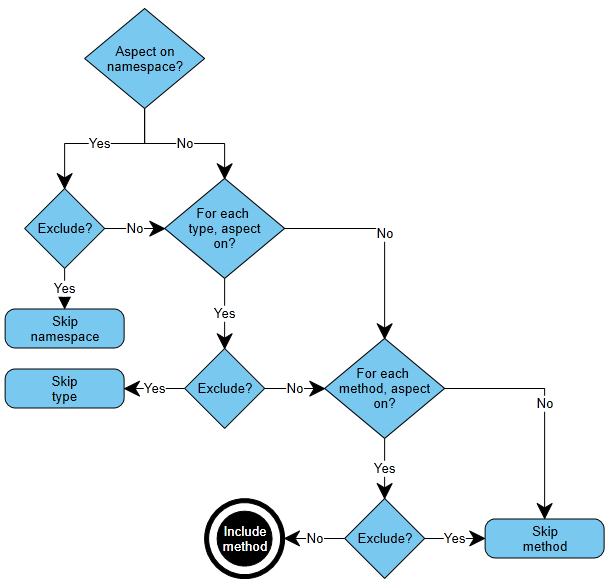
\includegraphics[scale=1.0]{AspectLogicalInclusion.PNG}
  \centering
  \caption{Logical Inclusion\label{logical_inclusion}}
\end{figure}

If no aspect is applied on the assembly, that does not necessarily mean no aspect is applied anywhere, the aspect might still be applied on any given class or method.

The take away from the above diagram, is that Buffalo first checks if an aspect is applied to the target, then check if it is set to be excluded. At the end it will end up with a list of methods that should be CIL modified.

\section{Aspect Interface}

Figure~\ref{uml01} shows the relationship of various aspect types in Buffalo. This is used by Buffalo to identify aspects during reflection.

\begin{figure}[H]
  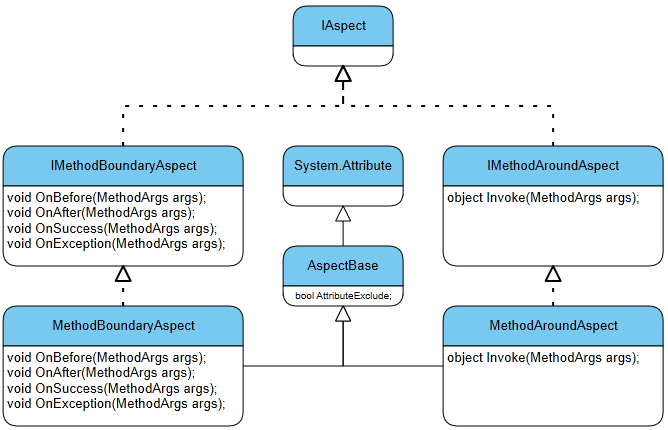
\includegraphics[scale=1.0]{Uml01.PNG}
  \centering
  \caption{Aspect Inheritance\label{uml01}}
\end{figure}

All aspects ultimately implements the IAspect interface, therefore it can be reasoned that for all the public types in an assembly, if it implements IAspect, then it must be an aspect itself.

All aspects have a property named AttributeExclude, if set to true then the annotated target will not be included in the weaving.

Buffalo supports more than one aspect applied at any given level. This will allow developers more flexibility while developing multiple aspects and applying them as needed.

Furthermore, by default, an aspect will be automatically excluded from applying to itself. This is implemented to prevent stack overflow in some cases. Although argument can be made that an aspect should be able to be applied to a different aspect, however that is not currently implemented in Buffalo.

\section{MethodArgs}

As mentioned above, when all is said and done, an aspect ultimately gets injected into each \textit{individual} method. When developing an aspect, a developer can access various information about the target method, via the MethodArgs object passed in as parameter to the aspect. Currently the full method signature, the method name, return type and parameter list including parameter name, type and value are captured for each target method.

The parameter list capturing is especially of interest, it enables developer to peek inside the method that is executing at various point and inspect its parameter values. This will be useful in case such as exception handling, where it will be useful to actually see what the values were at the time of the exception.

\section{Visual Studio Solution Structure}

Originally Buffalo was implemented as one executable, that includes the various aspects and the program that initiates the weaving. It was later on separated into two assemblies. One is a class library that contains the actual implementation. Another is a command line executable that calls into the class library to perform the weaving, as shown in figure~\ref{solutionexplorer}. This separation is necessary so developer can perform weaving from the command line or hook into MS-Build if necessary. 

To actually write the aspect, developer only need to reference the class library which is much cleaner than referencing an executable.

\begin{figure}[H]
  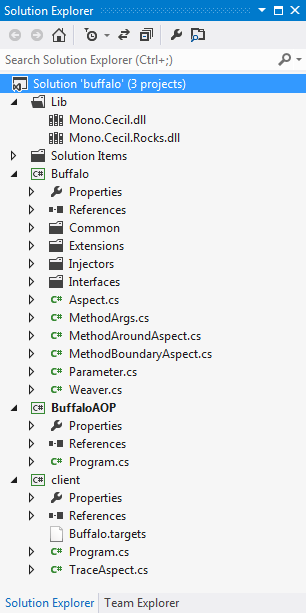
\includegraphics[scale=1.0]{SolutionExplorer.PNG}
  \centering
  \caption{Solution Structure\label{solutionexplorer}}
\end{figure}

The client project shown above is a simple program included in the solution for testing. The full source code is included in Appendix A.

\section{Implementation Overview}

The overall implementation process can be illustrated as figure~\ref{implementation_overview}, where the first step of finding all eligible methods using the logical diagram mentioned in figure~\ref{logical_inclusion}.

\begin{figure}[H]
  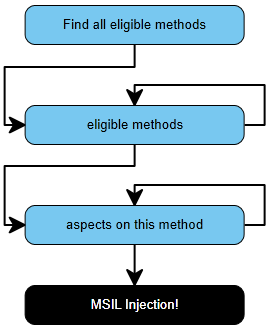
\includegraphics[scale=1.0]{ImplementationOverview3.PNG}
  \centering
  \caption{Implementation Overview\label{implementation_overview}}
\end{figure}

Then it loops through each eligible method, and for each aspect associated with the eligible method do the CIL injection. The actual injection phrase depends on the type of aspect.

\section{MethodBoundaryAspect Implementation Detail}

Each type of aspect has its own injector that implements the IInjectable interface. This interface contains only one method contract - Inject(..). It takes the list of eligible methods and inject the appropriate aspect to them.

MethodBoundaryAspect is pretty straightforward to implement. Take the following hello world example, wrapped in a try..catch..finally block as mentioned previously:

\begin{lstlisting}[caption={SayHello function}, label=sayhello]
public void SayHello()
{
   try{
       Console.WriteLine(“Hello World!”);
   }catch(Exception ex){
   }finally{
   }
}
\end{lstlisting}

The generated CIL is shown in figure~\ref{methodboundaryB4}. For ease of display the CIL has been cleaned up a bit:

\begin{lstlisting}[caption={CIL generated for sample C\# function}, label=methodboundaryB4]
.try
{
   .try
   {
      IL_0002: Ldstr "Hello World!"
      IL_0007: call void [mscorlib]System.Console::WriteLine(string)
      IL_000e: leave.s IL0015
   }
   catch [mscorlib]System.Exception
   {
      IL_0010: stloc.0
      IL_0013: leave.s IL_0015
   }
   IL_0015: leave.s IL_001c
}
finally
{
   IL_001a: endfinally
}
IL_001c: ret
\end{lstlisting}

Figure~\ref{methodboundaryB4} shows the standard emission of the CLR when it encounters the try-catch-finally statement. In CLR there is a concept of the protected region, where each region is associated with a handler. A try-catch-finally is actually encapsulated in two such regions: a catch and a finally. From here it can be easily figured out where to inject the various boundary aspects, as shown in figure~\ref{methodboundary02}.

\begin{figure}[H]
  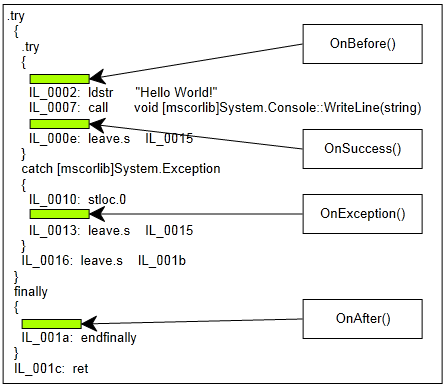
\includegraphics[scale=1.0]{MethodBoundaryOverview.PNG}
  \centering
  \caption{CIL Interception Points\label{methodboundary02}}
\end{figure}

The actual implementation is in provided in Listing~\ref{../buffalo/Injectors/MethodBoundaryInjector.cs}

\section{MethodAroundAspect Implementation Detail}

The Around aspect on the other hand is a much more complicated compared to the Boundary aspect.

MethodAroundAspect implements IMethodAroundAspect which has the following contract:

\begin{lstlisting}[caption={IMethodAroundAspect Contract}, label=aroundcontract]
internal interface IMethodAroundAspect : IAspect
{
	void Invoke(MethodArgs args)
}
\end{lstlisting}

When developing an aspect a Proceed() can be issued to signal a call back into the original method. The steps taken to implement MethodAroundAspect in CIL is roughly as follow:

\begin{enumerate}
	\item Create a replacement for the annotated function with exactly the same method signature.
	\item Create and store a variable pointing to the aspect.
	\item Copy all parameters from original method to the newly created replacement function.
	\item Create a variable to hold MethodArgs.
	\item Issue a call to Invoke() from the replacement function, passing in the MethodArgs variable.
	\item Handle the return value appropriately.
	\begin{enumerate}
		\item If original method returns non void type, put the return value back on the stack.
		\item If original method returns void, we need to discard the return value from Invoke().
	\end{enumerate}
	\item Handle Proceed() that might be issued from inside the Invoke().
	\begin{enumerate}
		\item Load all the parameters onto the stack.
		\item Call back into the original method.
		\item Handle the return value appropriately.
	\end{enumerate}
	\item Modify all calls from original method to the replacement method.
\end{enumerate}

As figure~\ref{around_overview} shown, the actual calling of either the original or replacement method is abstracted away. This is also a testament of the saying in Software Engineering that "anything can be resolved by another layer of abstraction".

Another important distinction is that MethodAroundAspect currently can be applied only on the method level, and that it should be applied to one method only. This is by design because a replacement method might not be appropriate to replace more than one method. Especially if it is applied on the assembly level, all the public methods will be replaced by a single replacement method!

The actual implementation of MethodAroundAspect is in provided in Listing~\ref{../buffalo/Injectors/MethodAroundInjector.cs}

\section{MethodArgs Implementation Detail}

When developing an aspect, information about the target method can be accessed. To achieve that MethodArgs is used. This is the object passed into each aspect. During the weaving, an instance of MethodArgs is created, with all properties assembled dynamically to capture the information of the current executing method. MethodArgs is then passed as parameter into each of the aspect.

Being able to capture some information about the annotated methods will be useful. For example, in case of a profiling aspect, those information about the method at the time it was access will be helpful. Being able to look at the parameter values in case of error will also be extremely useful in case of debugging.

An early implementation instantiated a distinct instance of MethodArgs for each boundary aspects. Later on as an optimization only one instance is instantiated at the beginning of the method body and that instance is used in all the boundary aspects for a target method.

An example of how to use MethodArgs is presented in the user manual.
